% !TEX encoding = UTF-8 Unicode
\section{Preventivo}
	\subsection{Dettaglio fasi}
		\subsubsection{Fase A}
			\paragraph{Suddivisione lavoro}
				Nella \insphase{Fase A} ogni componente del gruppo \groupname{} coprirà i seguenti ruoli:
				\begin{table}
					\begin{center}
						\begin{tabular}{| l | c | c | c | c | c | c | c |}
							\hline
							Componente 					& PM		& Am 		& An 		& Pt 		& Pm 		& Ve 		& Ore Totali componente \\ \hline
							
							Bigarella Chiara 			& - 		& 5 		& 30 		& - 		& - 		& 8 		& 43 \\
							Bucco Riccardo 				& - 		& 5 		& 30 		& - 		& -			& 8 		& 43 \\
							Carlon Chiara	 			& - 		& 6 		& 9 		& - 		& - 		& 17 		& 32 \\
							Dal Bianco Davide 			& - 		& 14 		& 25 		& - 		& - 		& 5 		& 44 \\
							Moretto Alessandro 			& 25 		& - 		& 9 		& - 		& - 		& 8 		& 42 \\
							Pavanello Fabio Matteo	 	& - 		& 5 		& 6 		& - 		& - 		& 23 		& 34 \\
							Rubin Marco					& 7 		& 19 		& - 		& - 		& - 		& 8 		& 34 \\ \hline \hline
							
							Ore Totali Ruolo 			& 32 		& 54 		& 109 		& - 		& - 		& 77 		& 272\\ \hline
						\end{tabular}
					\end{center}
					\caption{Suddivisione ore di lavoro Fase A}
				\end{table}
				Riassumendo con un Bar Chart:
				\begin{figure}\centering
					%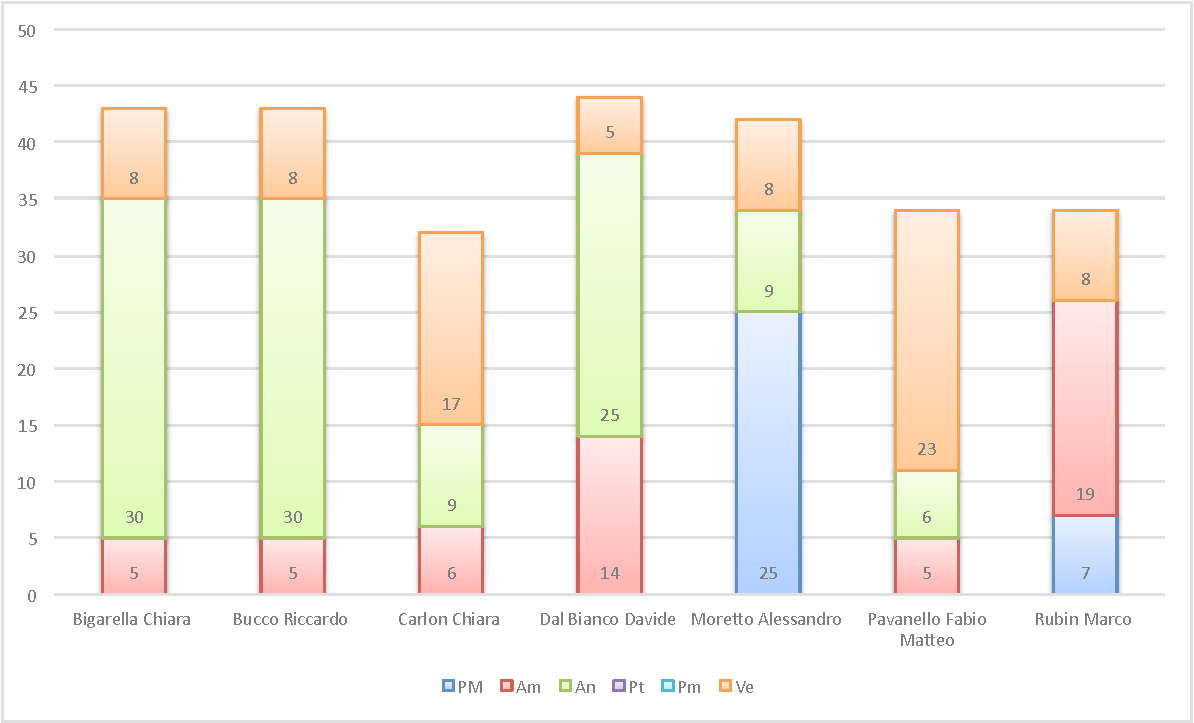
\includegraphics[width=\textwidth]{PianoDiProgetto/Pics/ChartOreFaseA.png}
					\caption{Bar Chart ore persona Fase A}
				\end{figure}
			\paragraph{Prospetto economico}
				Nella \insphase{Fase A} il costo di ogni ruolo è il seguente:
				\begin{table}
					\begin{center}
						\begin{tabular}{| l | c | c |}
							\hline
							Ruolo 			& Ore 	& Costi  \\ \hline
							
							Product Manager	& 32 		& \euro{} 960 	\\
							Amministratore 		& 54 		& \euro{} 1080 	\\
							Analista	 		& 109 		& \euro{} 2725 	\\
							Progettista 		& - 		& \euro{} -  	\\
							Programmatore		& - 		& \euro{} - 	\\
							Verificatore		& 77 		& \euro{} 1155 	\\ \hline \hline
							
							Totale	 		& 272 		& \euro{} 5920 	\\ \hline
						\end{tabular}
					\end{center}
					\caption{Costi per ruolo Fase A}
				\end{table}
				Riassumendo le ore per ruolo con un Cake Chart:
				\begin{figure}\centering
					%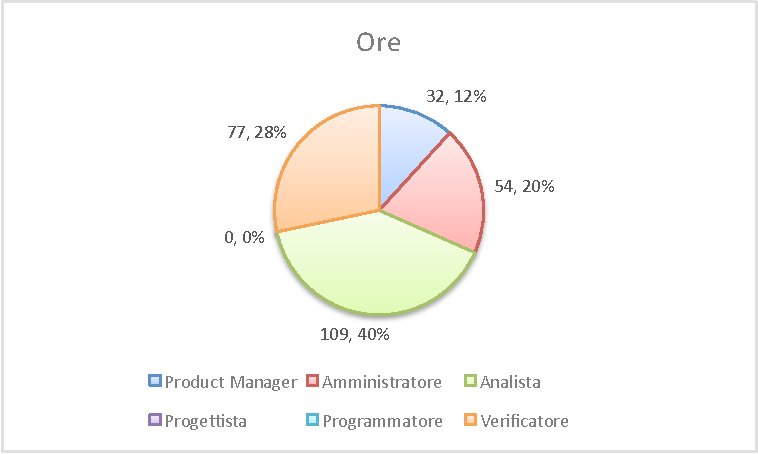
\includegraphics[width=\textwidth]{PianoDiProgetto/Pics/ChartTotOreFaseA.png}
					\caption{Cake Chart ore per ruolo Fase A}
				\end{figure}
				Riassumendo i costi per ruolo con un Cake Chart:
				\begin{figure}\centering
					%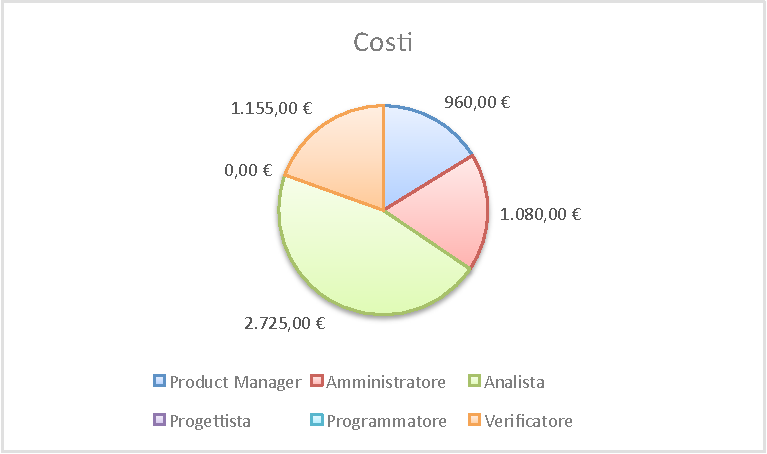
\includegraphics[width=\textwidth]{PianoDiProgetto/Pics/ChartTotCostiFaseA.png}
					\caption{Cake Chart costi per ruolo Fase A}
				\end{figure}
		\subsubsection{Fase AD}
			\paragraph{Suddivisione lavoro}
				Nella \insphase{Fase AD} ogni componente del gruppo \groupname{} coprirà i seguenti ruoli:
				\begin{table}
					\begin{center}
						\begin{tabular}{| l | c | c | c | c | c | c | c |}
							\hline
							Componente 					& PM		& Am 		& An 		& Pt 		& Pm 		& Ve 		& Ore Totali componente \\ \hline
							
							Bigarella Chiara 			& - 		& 7 		& - 		& - 		& - 		& 5 		& 12 \\
							Bucco Riccardo 				& - 		& 6 		& - 		& - 		& -			& 7 		& 13 \\
							Carlon Chiara	 			& 7 		& - 		& 3 		& - 		& - 		& 2 		& 12 \\
							Dal Bianco Davide 			& - 		& 6 		& - 		& - 		& - 		& 5 		& 11 \\
							Moretto Alessandro 			& - 		& - 		& 3 		& - 		& - 		& 8 		& 11 \\
							Pavanello Fabio Matteo	 	& - 		& - 		& 3 		& - 		& - 		& 10 		& 13 \\
							Rubin Marco					& - 		& - 		& 3 		& - 		& - 		& 10 		& 13 \\ \hline \hline
							
							Ore Totali Ruolo 			& 7 		& 19 		& 12 		& - 		& - 		& 47 		& 85\\ \hline
						\end{tabular}
					\end{center}
					\caption{Suddivisione ore di lavoro Fase AD}
				\end{table}
				Riassumendo con un Bar Chart:
				\begin{figure}\centering
					%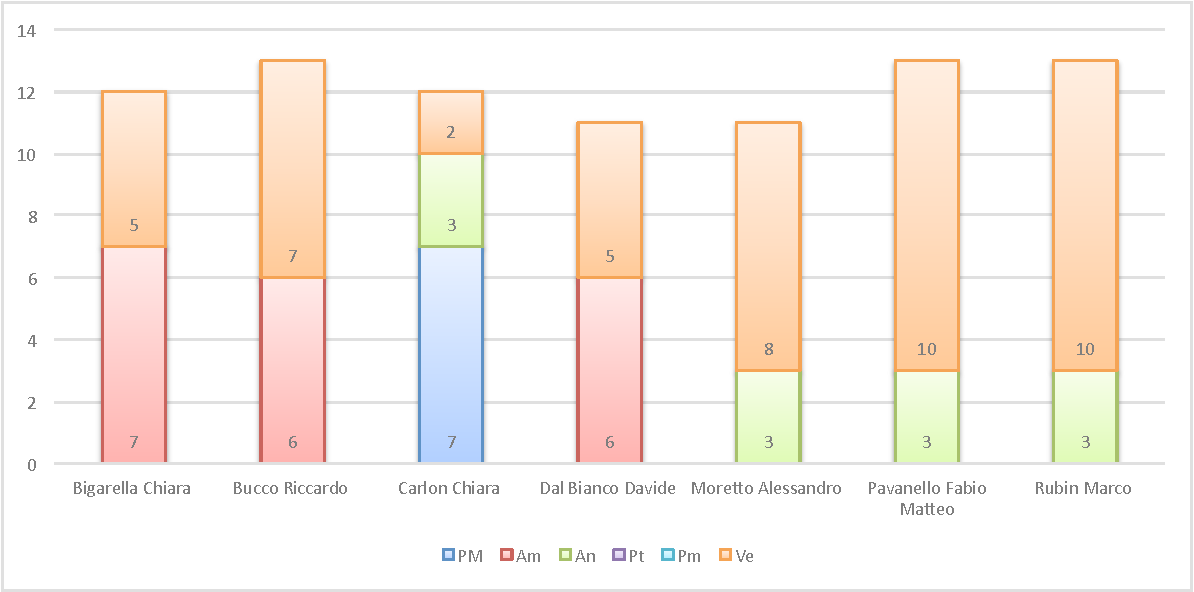
\includegraphics[width=\textwidth]{PianoDiProgetto/Pics/ChartOreFaseAD.png}
					\caption{Bar Chart ore persona Fase AD}
				\end{figure}
			\paragraph{Prospetto economico}
				Nella \insphase{Fase AD} il costo di ogni ruolo è il seguente:
				\begin{table}
					\begin{center}
						\begin{tabular}{| l | c | c |}
							\hline
							Ruolo 				& Ore 		& Costi  \\ \hline
							
							Product Manager		& 7 		& \euro{} 210 	\\
							Amministratore 		& 19 		& \euro{} 380 	\\
							Analista	 		& 12 		& \euro{} 300 	\\
							Progettista 		& - 		& \euro{} -  	\\
							Programmatore		& - 		& \euro{} - 	\\
							Verificatore		& 47 		& \euro{} 705 	\\ \hline \hline
							
							Totale	 			& 85 		& \euro{} 1595 	\\ \hline
						\end{tabular}
					\end{center}
					\caption{Costi per ruolo Fase AD}
				\end{table}
				Riassumendo le ore per ruolo con un Cake Chart:
				\begin{figure}\centering
					%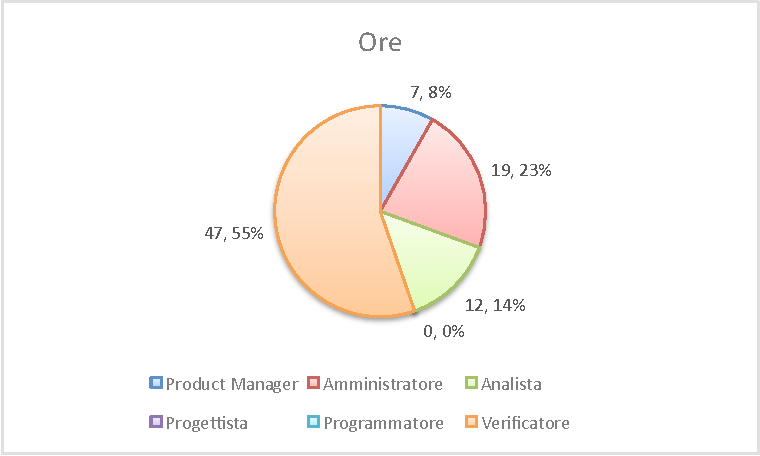
\includegraphics[width=\textwidth]{PianoDiProgetto/Pics/ChartTotOreFaseAD.png}
					\caption{Cake Chart ore per ruolo Fase AD}
				\end{figure}
				Riassumendo i costi per ruolo con un Cake Chart:
				\begin{figure}\centering
					%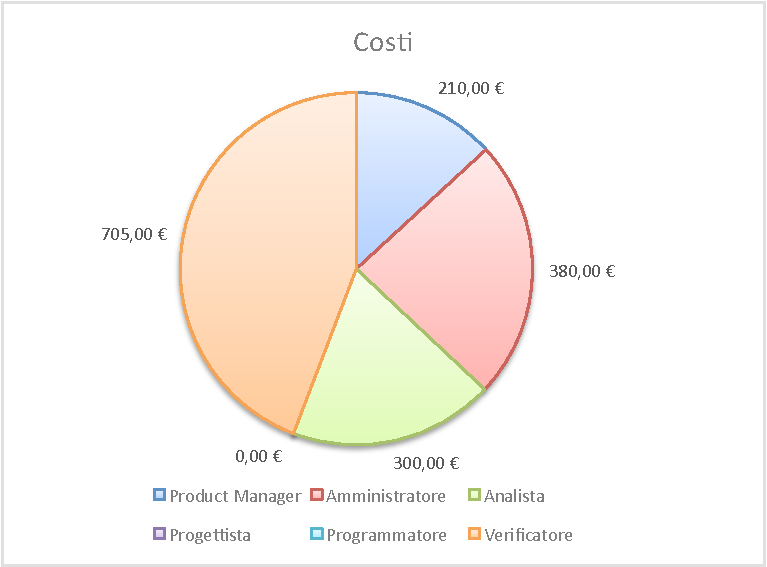
\includegraphics[width=\textwidth]{PianoDiProgetto/Pics/ChartTotCostiFaseAD.png}
					\caption{Cake Chart costi per ruolo Fase AD}
				\end{figure}
		\subsubsection{Fase PA}
			\paragraph{Suddivisione lavoro}
				Nella \insphase{Fase PA} ogni componente del gruppo \groupname{} coprirà i seguenti ruoli:
				\begin{table}
					\begin{center}
						\begin{tabular}{| l | c | c | c | c | c | c | c |}
							\hline
							Componente 					& PM		& Am		 	& An 	& Pt 		& Pm 		& Ve 		& Ore Totali componente \\ \hline
							
							Bigarella Chiara 			& - 		& - 		& 10 		& 17 		& - 		& 6 		& 33 \\
							Bucco Riccardo 				& 15 		& - 		& - 		& 15 		& -			& 5 		& 35 \\
							Carlon Chiara	 			& - 		& 7 		& 12 		& - 		& - 		& 9 		& 28 \\
							Dal Bianco Davide 			& - 		& - 		& - 		& 25 		& - 		& - 		& 25 \\
							Moretto Alessandro 			& - 		& 3 		& 10 		& 15 		& - 		& 2 		& 30 \\
							Pavanello Fabio Matteo	 	& - 		& - 		& 25 		& - 		& - 		& - 		& 25 \\
							Rubin Marco					& 9 		& - 		& 12 		& - 		& - 		& 7 		& 28 \\ \hline \hline
							
							Ore Totali Ruolo 			& 24 		& 10 		& 69 		& 72 		& - 		& 29 		& 204\\ \hline
						\end{tabular}
					\end{center}
					\caption{Suddivisione ore di lavoro Fase PA}
				\end{table}
				Riassumendo con un Bar Chart:
				\begin{figure}\centering
					%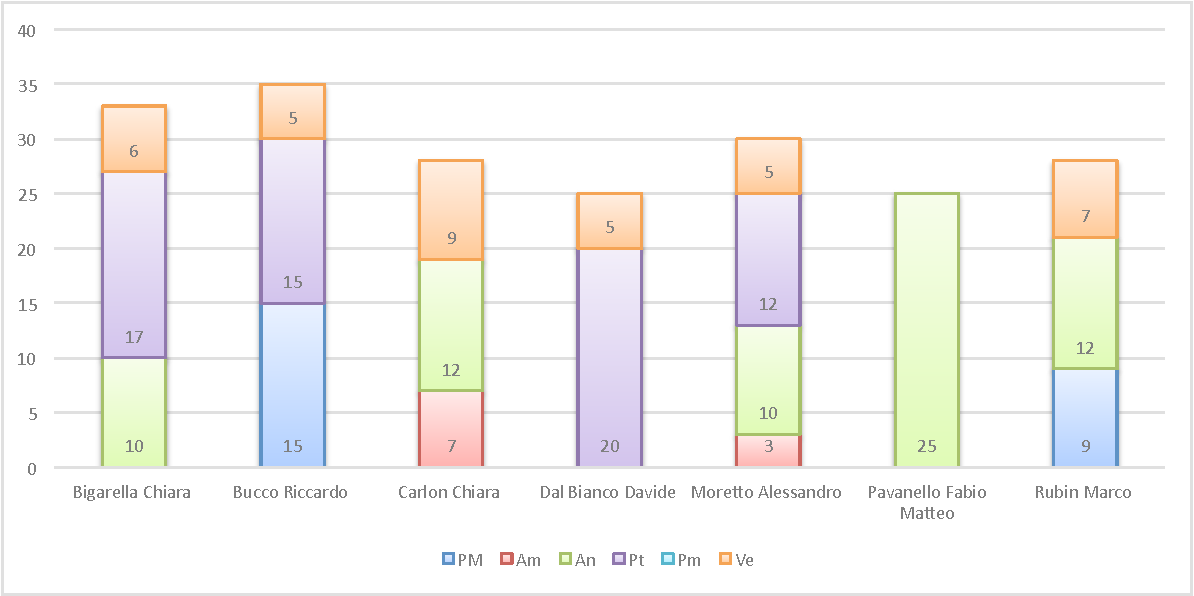
\includegraphics[width=\textwidth]{PianoDiProgetto/Pics/ChartOreFasePA.png}
					\caption{Bar Chart ore persona Fase PA}
				\end{figure}
			\paragraph{Prospetto economico}
				Nella \insphase{Fase PA} il costo di ogni ruolo è il seguente:
				\begin{table}
					\begin{center}
						\begin{tabular}{| l | c | c |}
							\hline
							Ruolo 				& Ore 		& Costi  \\ \hline
							
							Product Manager		& 24 		& \euro{} 720 	\\
							Amministratore 		& 10 		& \euro{} 200 	\\
							Analista	 		& 69 		& \euro{} 1725 	\\
							Progettista 		& 72 		& \euro{} 1584  	\\
							Programmatore		& - 		& \euro{} - 	\\
							Verificatore		& 29 		& \euro{} 435 	\\ \hline \hline
							
							Totale	 			& 204 		& \euro{} 4664 	\\ \hline
						\end{tabular}
					\end{center}
					\caption{Costi per ruolo Fase PA}
				\end{table}
				Riassumendo le ore per ruolo con un Cake Chart:
				\begin{figure}\centering
					%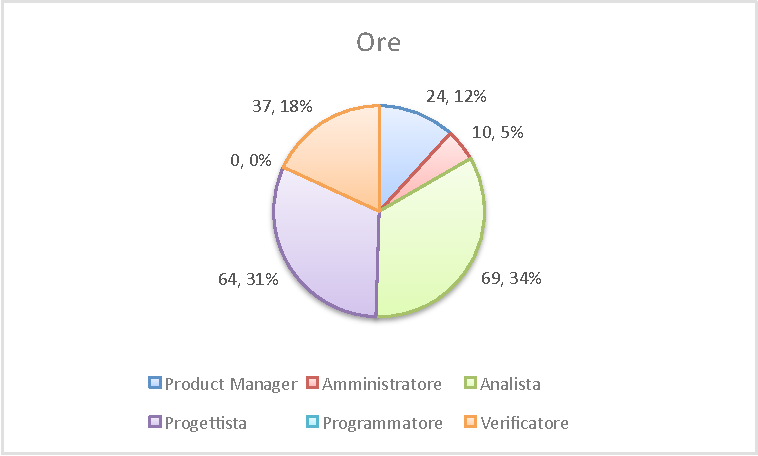
\includegraphics[width=\textwidth]{PianoDiProgetto/Pics/ChartTotOreFasePA.png}
					\caption{Cake Chart ore per ruolo Fase PA}
				\end{figure}
				Riassumendo i costi per ruolo con un Cake Chart:
				\begin{figure}\centering
					%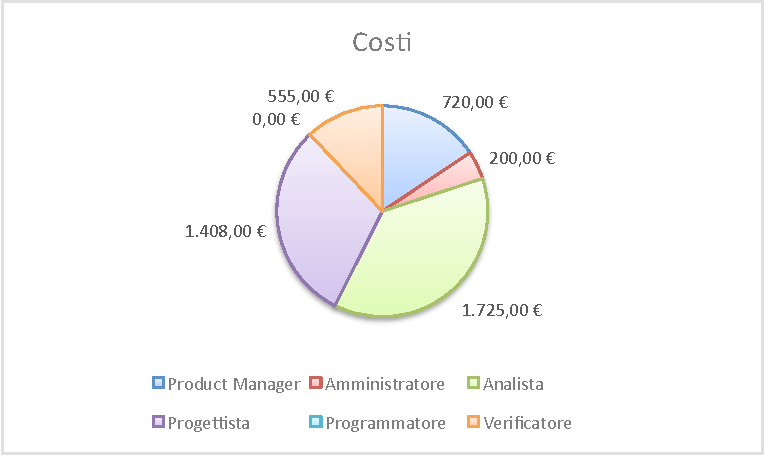
\includegraphics[width=\textwidth]{PianoDiProgetto/Pics/ChartTotCostiFasePA.png}
					\caption{Cake Chart costi per ruolo Fase PA}
				\end{figure}
		\subsubsection{Fase PROB}
			\paragraph{Suddivisione lavoro}
				Nella \insphase{Fase PROB} ogni componente del gruppo \groupname{} coprirà i seguenti ruoli:
				\begin{table}
					\begin{center}
						\begin{tabular}{| l | c | c | c | c | c | c | c |}
							\hline
							Componente 					& PM		& Am 		& An 		& Pt 		& Pm 		& Ve 		& Ore Totali componente \\ \hline
							
							Bigarella Chiara 			& - 		& - 		& - 		& 9 		& 16 		& 6 		& 31 \\
							Bucco Riccardo 				& - 		& - 		& - 		& 7 		& 17		& 10 		& 34 \\
							Carlon Chiara	 			& - 		& - 		& 13 		& - 		& 13 		& 4 		& 30 \\
							Dal Bianco Davide 			& 17 		& - 		& - 		& 13 		& - 		& 3 		& 33 \\
							Moretto Alessandro 			& - 		& 5 		& - 		& 17 		& 4 		& 8 		& 34 \\
							Pavanello Fabio Matteo	 	& - 		& - 		& 12 		& - 		& 10 		& 11 		& 33 \\
							Rubin Marco					& - 		& 4 		& - 		& 17 		& - 		& 8 		& 29 \\ \hline \hline
							
							Ore Totali Ruolo 			& 17 		& 9 		& 25 		& 63 		& 60 		& 50 		& 224	\\ \hline
						\end{tabular}
					\end{center}
					\caption{Suddivisione ore di lavoro Fase PROB}
				\end{table}
				Riassumendo con un Bar Chart:
				\begin{figure}\centering
					%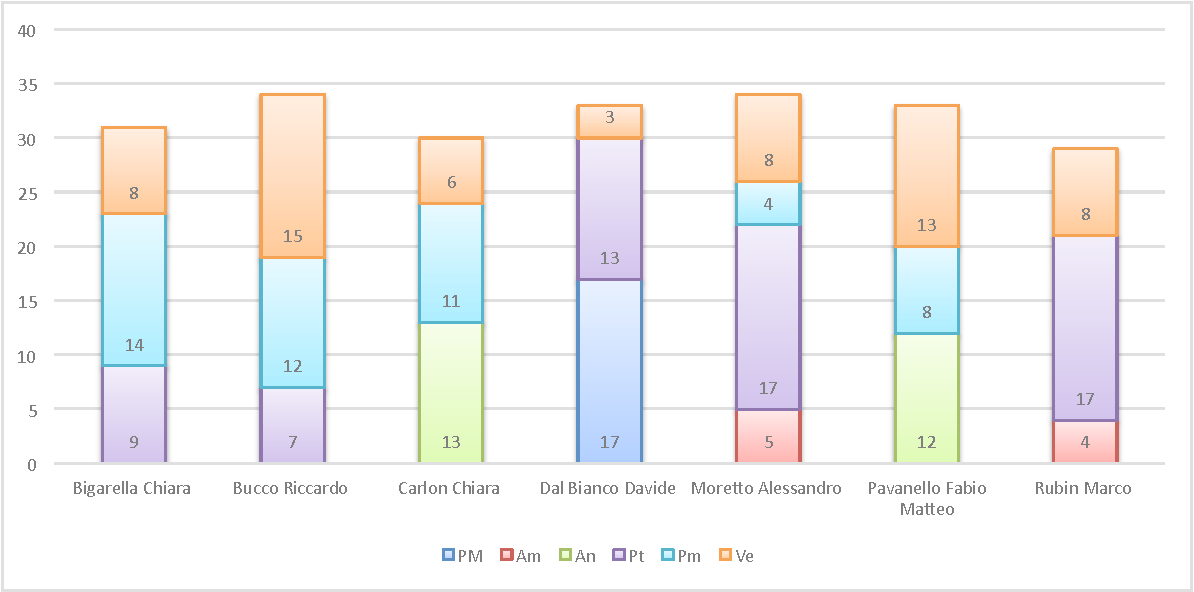
\includegraphics[width=\textwidth]{PianoDiProgetto/Pics/ChartOreFasePROB.png}
					\caption{Bar Chart ore persona Fase PROB}
				\end{figure}
			\paragraph{Prospetto economico}
				Nella \insphase{Fase PROB} il costo di ogni ruolo è il seguente:
				\begin{table}
					\begin{center}
						\begin{tabular}{| l | c | c |}
							\hline
							Ruolo 				& Ore 		& Costi  \\ \hline
							
							Product Manager		& 17 		& \euro{} 510 	\\
							Amministratore 		& 9 		& \euro{} 180 	\\
							Analista	 		& 25 		& \euro{} 625 	\\
							Progettista 		& 63 		& \euro{} 1386  	\\
							Programmatore		& 60 		& \euro{} 900 	\\
							Verificatore		& 50 		& \euro{} 750 	\\ \hline \hline
							
							Totale	 			& 224 		& \euro{} 4351 	\\ \hline
						\end{tabular}
					\end{center}
					\caption{Costi per ruolo Fase PROB}
				\end{table}
				Riassumendo le ore per ruolo con un Cake Chart:
				\begin{figure}\centering
					%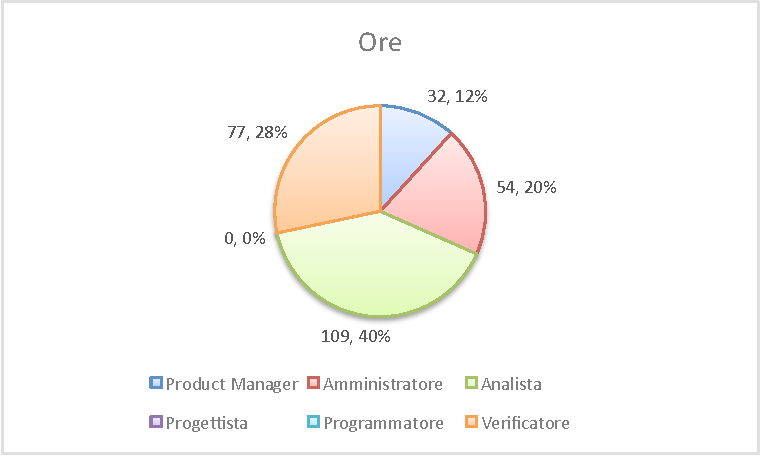
\includegraphics[width=\textwidth]{PianoDiProgetto/Pics/ChartTotOreFasePROB.png}
					\caption{Cake Chart ore per ruolo Fase PROB}
				\end{figure}
				Riassumendo i costi per ruolo con un Cake Chart:
				\begin{figure}\centering
					%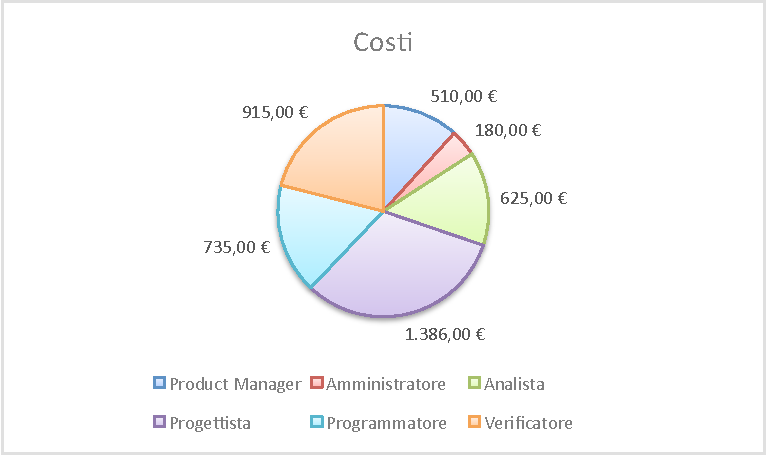
\includegraphics[width=\textwidth]{PianoDiProgetto/Pics/ChartTotCostiFasePROB.png}
					\caption{Cake Chart costi per ruolo Fase PROB}
				\end{figure}
		\subsubsection{Fase PRD}
			\paragraph{Suddivisione lavoro}
				Nella \insphase{Fase PRD} ogni componente del gruppo \groupname{} coprirà i seguenti ruoli:
				\begin{table}
					\begin{center}
						\begin{tabular}{| l | c | c | c | c | c | c | c |}
							\hline
							Componente 					& PM		& Am	 	& An 		& Pt 		& Pm 		& Ve 		& Ore Totali componente \\ \hline
							
							Bigarella Chiara 			& 10 		& - 		& - 		& - 		& 3 		& - 		& 13 \\
							Bucco Riccardo 				& - 		& - 		& - 		& - 		& 2			& 12 		& 14 \\
							Carlon Chiara	 			& - 		& 2 		& - 		& 4 		& 2 		& 8 		& 16 \\
							Dal Bianco Davide 			& - 		& - 		& - 		& - 		& 6 		& 7 		& 13 \\
							Moretto Alessandro 			& - 		& - 		& 13 		& - 		& - 		& - 		& 13 \\
							Pavanello Fabio Matteo	 	& - 		& - 		& - 		& - 		& 8 		& 6 		& 14 \\
							Rubin Marco					& - 		& 3 		& - 		& 6 		& 9 		& - 		& 18 \\ \hline \hline
							
							Ore Totali Ruolo 			& 10 		& 5 		& 13 		& 10 		& 30 		& 33 		& 101\\ \hline
						\end{tabular}
					\end{center}
					\caption{Suddivisione ore di lavoro Fase PRD}
				\end{table}
				Riassumendo con un Bar Chart:
				\begin{figure}\centering
					%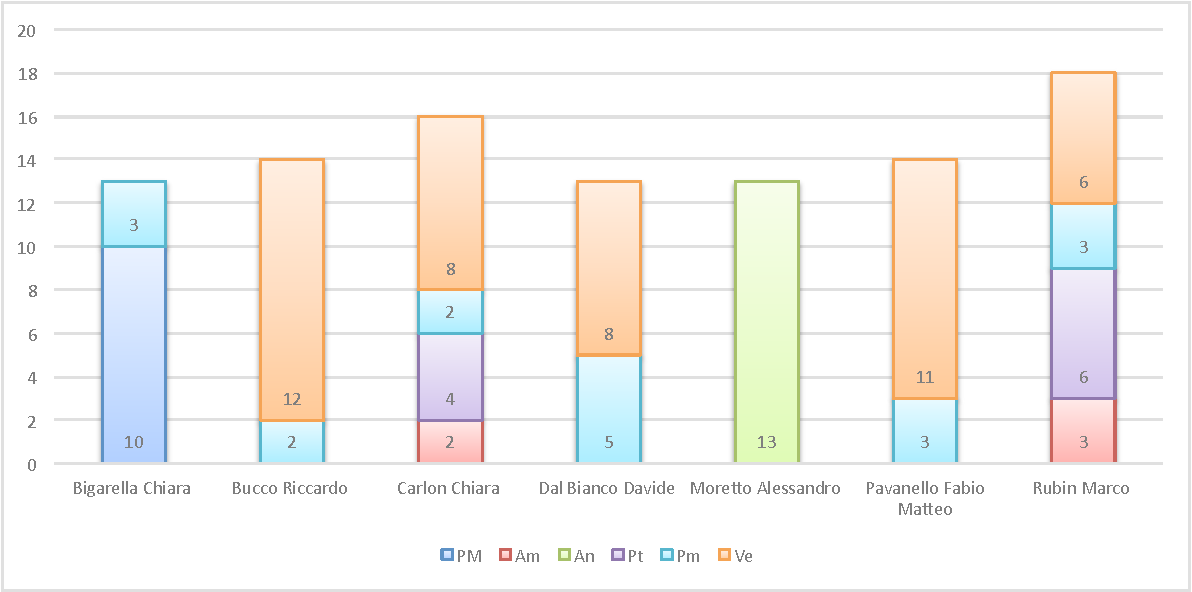
\includegraphics[width=\textwidth]{PianoDiProgetto/Pics/ChartOreFasePRD.png}
					\caption{Bar Chart ore persona Fase PRD}
				\end{figure}
			\paragraph{Prospetto economico}
				Nella \insphase{Fase PRD} il costo di ogni ruolo è il seguente:
				\begin{table}
					\begin{center}
						\begin{tabular}{| l | c | c |}
							\hline
							Ruolo 				& Ore 		& Costi  \\ \hline
							
							Product Manager		& 10 		& \euro{} 300 	\\
							Amministratore 		& 5 		& \euro{} 100 	\\
							Analista	 		& 13 		& \euro{} 325 	\\
							Progettista 		& 10 		& \euro{} 220  	\\
							Programmatore		& 30 		& \euro{} 450 	\\
							Verificatore		& 33 		& \euro{} 495 	\\ \hline \hline
							
							Totale	 			& 101 		& \euro{} 1890 	\\ \hline
						\end{tabular}
					\end{center}
					\caption{Costi per ruolo Fase PRD}
				\end{table}
				Riassumendo le ore per ruolo con un Cake Chart:
				\begin{figure}\centering
					%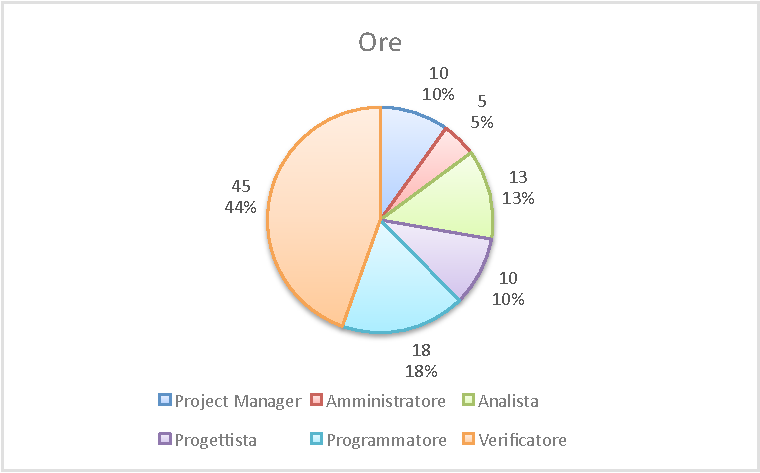
\includegraphics[width=\textwidth]{PianoDiProgetto/Pics/ChartTotOreFasePRD.png}
					\caption{Cake Chart ore per ruolo Fase PRD}
				\end{figure}
				Riassumendo i costi per ruolo con un Cake Chart:
				\begin{figure}\centering
					%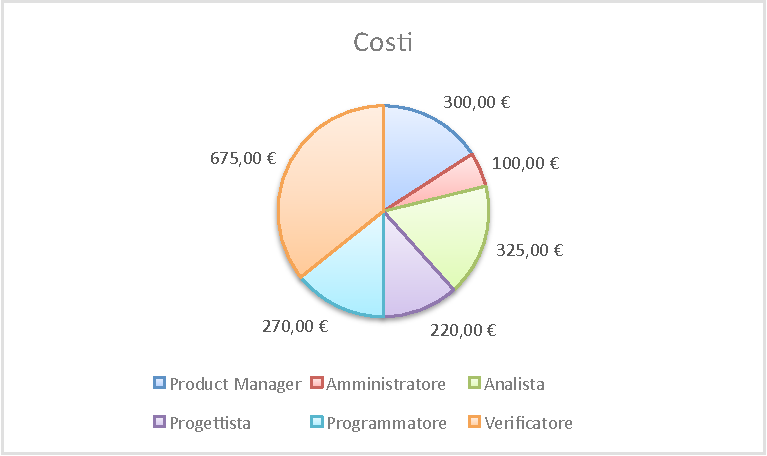
\includegraphics[width=\textwidth]{PianoDiProgetto/Pics/ChartTotCostiFasePRD.png}
					\caption{Cake Chart costi per ruolo Fase PRD}
				\end{figure}
		\subsubsection{Fase PROP}
			\paragraph{Suddivisione lavoro}
				Nella \insphase{Fase PROP} ogni componente del gruppo \groupname{} coprirà i seguenti ruoli:
				\begin{table}
					\begin{center}
						\begin{tabular}{| l | c | c | c | c | c | c | c |}
							\hline
							Componente 					& PM		& Am 		& An 		& Pt 		& Pm 	& Ve 		& Ore Totali componente \\ \hline
							
							Bigarella Chiara 			& - 		& - 		& - 		& 6 		& - 		& 8 		& 14 \\
							Bucco Riccardo 				& - 		& - 		& - 		& 4 		& -			& 7 		& 11 \\
							Carlon Chiara	 			& - 		& 5 		& - 		& 10 		& - 		& 4 		& 18 \\
							Dal Bianco Davide 			& - 		& - 		& - 		& - 		& 17 		& 4 		& 21 \\
							Moretto Alessandro 			& - 		& - 		& - 		& - 		& 16 		& - 		& 16 \\
							Pavanello Fabio Matteo	 	& 13 		& - 		& - 		& - 		& 6 		& 3 		& 22 \\
							Rubin Marco					& - 		& - 		& 13 		& - 		& - 		& 4 		& 17 \\ \hline \hline
							
							Ore Totali Ruolo 			& 13 		& 5 		& 13 		& 20 		& 39 		& 29 		& 119\\ \hline
						\end{tabular}
					\end{center}
					\caption{Suddivisione ore di lavoro Fase PROP}
				\end{table}
				Riassumendo con un Bar Chart:
				\begin{figure}\centering
					%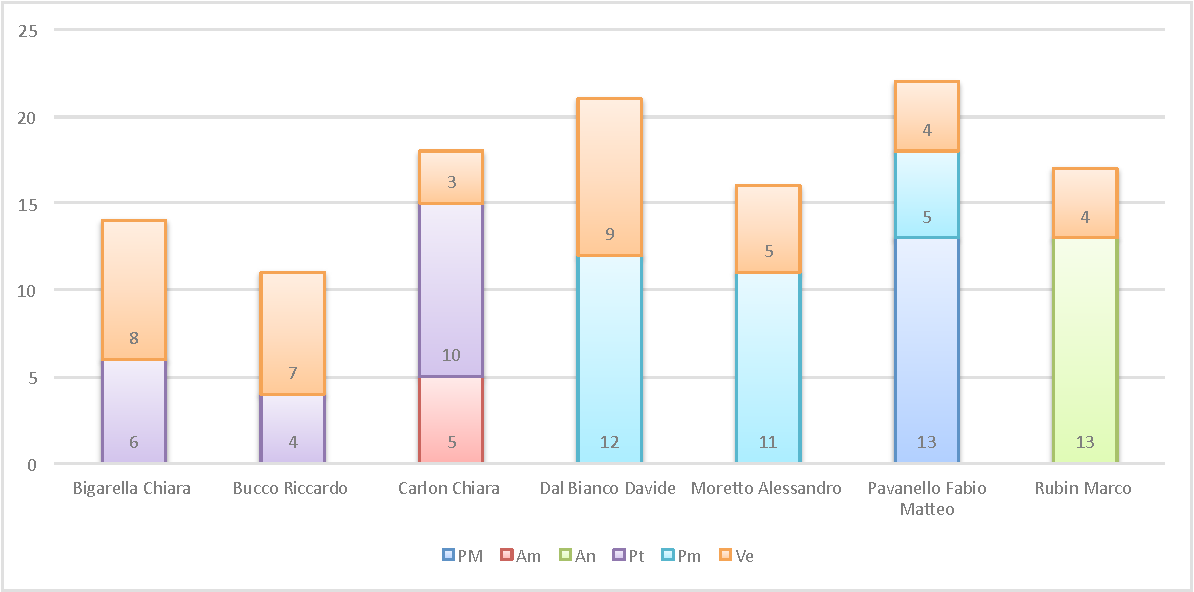
\includegraphics[width=\textwidth]{PianoDiProgetto/Pics/ChartOreFasePROP.png}
					\caption{Bar Chart ore persona Fase PROP}
				\end{figure}
			\paragraph{Prospetto economico}
				Nella \insphase{Fase PROP} il costo di ogni ruolo è il seguente:
				\begin{table}
					\begin{center}
						\begin{tabular}{| l | c | c |}
							\hline
							Ruolo 				& Ore 		& Costi  \\ \hline
							
							Product Manager		& 13 		& \euro{} 390 	\\
							Amministratore 		& 5 		& \euro{} 100 	\\
							Analista	 		& 13 		& \euro{} 325 	\\
							Progettista 		& 20 		& \euro{} 440  	\\
							Programmatore		& 39 		& \euro{} 585 	\\
							Verificatore		& 29 		& \euro{} 435 	\\ \hline \hline
							
							Totale	 			& 119 		& \euro{} 2275 	\\ \hline
						\end{tabular}
					\end{center}
					\caption{Costi per ruolo Fase PROP}
				\end{table}
				Riassumendo le ore per ruolo con un Cake Chart:
				\begin{figure}\centering
					%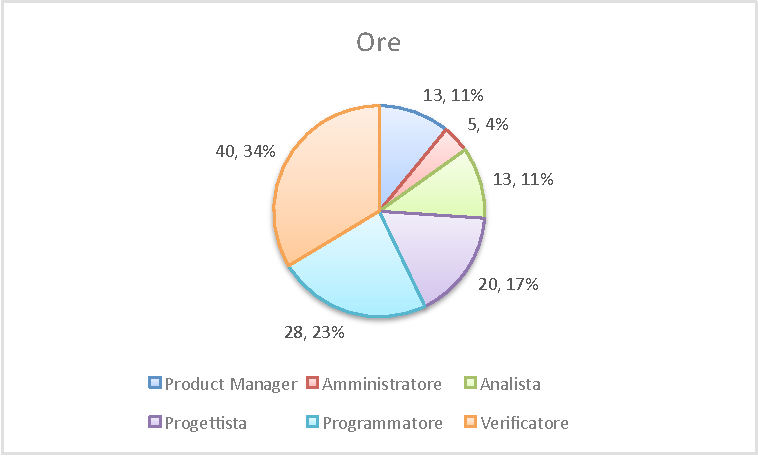
\includegraphics[width=\textwidth]{PianoDiProgetto/Pics/ChartTotOreFasePROP.png}
					\caption{Cake Chart ore per ruolo Fase PROP}
				\end{figure}
				Riassumendo i costi per ruolo con un Cake Chart:
				\begin{figure}\centering
					%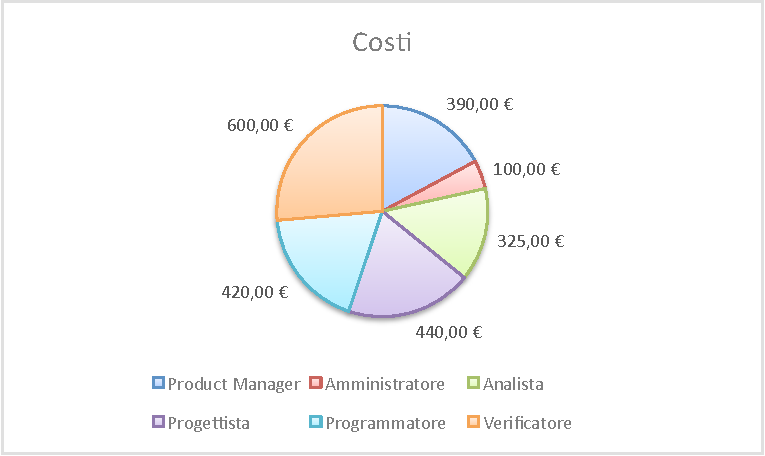
\includegraphics[width=\textwidth]{PianoDiProgetto/Pics/ChartTotCostiFasePROP.png}
					\caption{Cake Chart costi per ruolo Fase PROP}
				\end{figure}
		\subsubsection{Fase V}
			\paragraph{Suddivisione lavoro}
				Nella \insphase{Fase V} ogni componente del gruppo \groupname{} coprirà i seguenti ruoli:
				\begin{table}
					\begin{center}
						\begin{tabular}{| l | c | c | c | c | c | c | c |}
							\hline
							Componente 					& PM		& Am 		& An 		& Pt 		& Pm 		& Ve 		& Ore Totali componente \\ \hline
							
							Bigarella Chiara 			& - 		& - 		& - 		& - 		& 5 		& 9 		& 14 \\
							Bucco Riccardo 				& - 		& - 		& - 		& - 		& 7			& 4 		& 11 \\
							Carlon Chiara	 			& 10 		& - 		& - 		& - 		& - 		& 3 		& 13 \\
							Dal Bianco Davide 			& - 		& - 		& - 		& - 		& - 		& 13 		& 13 \\
							Moretto Alessandro 			& - 		& 3 		& - 		& - 		& - 		& 9 		& 12 \\
							Pavanello Fabio Matteo	 	& - 		& - 		& - 		& 9 		& - 		& 2 		& 11 \\
							Rubin Marco					& - 		& - 		& - 		& - 		& 5 		& 8 		& 13 \\ \hline \hline
							
							Ore Totali Ruolo 			& 10 		& 3 		& - 		& 9 		& 17 		& 48 		& 87\\ \hline
						\end{tabular}
					\end{center}
					\caption{Suddivisione ore di lavoro Fase V}
				\end{table}
				Riassumendo con un Bar Chart:
				\begin{figure}\centering
					%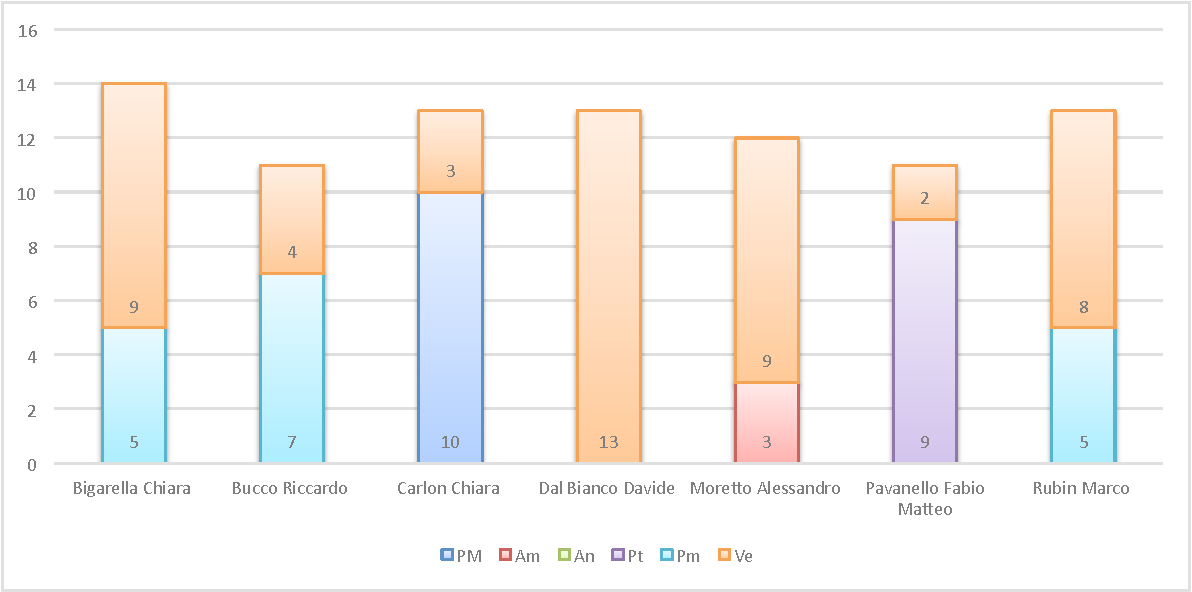
\includegraphics[width=\textwidth]{PianoDiProgetto/Pics/ChartOreFaseV.png}
					\caption{Bar Chart ore persona Fase V}
				\end{figure}
			\paragraph{Prospetto economico}
				Nella \insphase{Fase V} il costo di ogni ruolo è il seguente:
				\begin{table}
					\begin{center}
						\begin{tabular}{| l | c | c |}
							\hline
							Ruolo 				& Ore 		& Costi  \\ \hline
							
							Product Manager		& 10 		& \euro{} 300 	\\
							Amministratore 		& 3 		& \euro{} 60 	\\
							Analista	 		& - 		& \euro{} - 	\\
							Progettista 		& 9 		& \euro{} 198  	\\
							Programmatore		& 17 		& \euro{} 225 	\\
							Verificatore		& 48 		& \euro{} 720 	\\ \hline \hline
							
							Totale	 			& 87 		& \euro{} 1533 	\\ \hline
						\end{tabular}
					\end{center}
					\caption{Costi per ruolo Fase V}
				\end{table}
				Riassumendo le ore per ruolo con un Cake Chart:
				\begin{figure}\centering
					%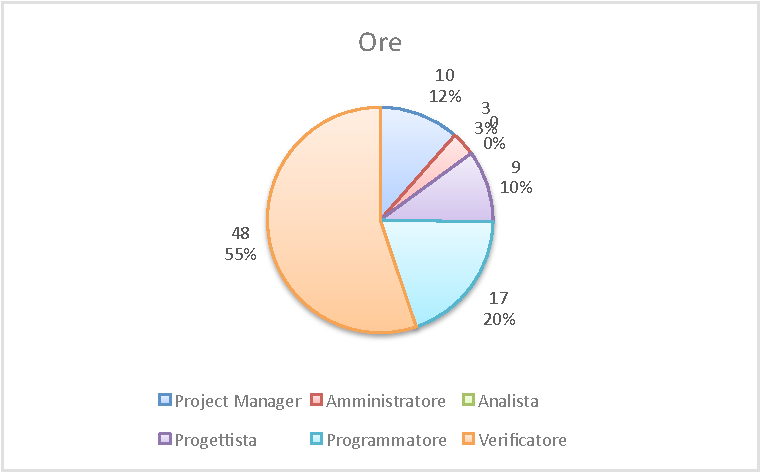
\includegraphics[width=\textwidth]{PianoDiProgetto/Pics/ChartTotOreFaseV.png}
					\caption{Cake Chart ore per ruolo Fase V}
				\end{figure}
				Riassumendo i costi per ruolo con un Cake Chart:
				\begin{figure}\centering
					%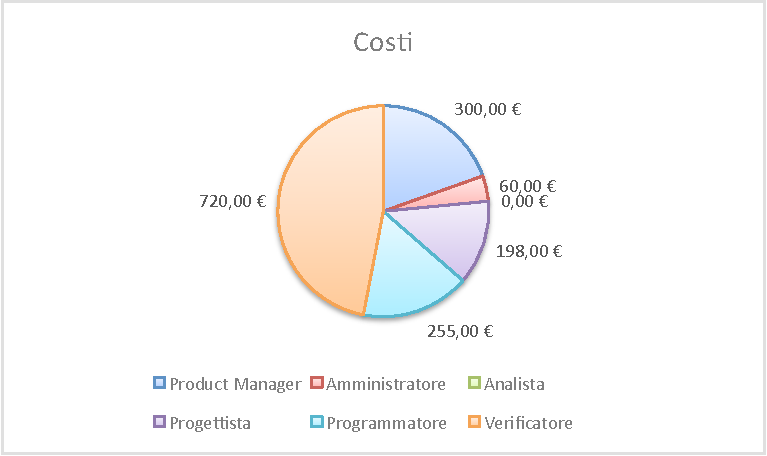
\includegraphics[width=\textwidth]{PianoDiProgetto/Pics/ChartTotCostiFaseV.png}
					\caption{Cake Chart costi per ruolo Fase V}
				\end{figure}
	\subsection{Resoconto}
		\subsubsection{Ore totali di investimento}
		Le ore di investimento sono le ore svolte non rendicontate. Durante la \insphase{Fase A} e la \insphase{Fase AD} le ore effettuate non sono a carico del proponente.
			\paragraph{Suddivisione lavoro}
				La suddivisione delle ore di investimento per ruolo di ogni componente del gruppo \groupname{} saranno le seguenti:
				\begin{table}
					\begin{center}
						\begin{tabular}{| l | c | c | c | c | c | c | c |}
							\hline
							Componente 					& PM		& Am 		& An 		& Pt 		& Pm 		& Ve 		& Ore Totali componente \\ \hline
							
							Bigarella Chiara 			& - 		& 12 		& 30 		& - 		& - 		& 13 		& 55 \\
							Bucco Riccardo 				& - 		& 11 		& 30 		& - 		& -			& 15 		& 56 \\
							Carlon Chiara	 			& 7 		& 6 		& 12 		& - 		& - 		& 19 		& 44 \\
							Dal Bianco Davide 			& - 		& 20 		& 25 		& - 		& - 		& 10 		& 55 \\
							Moretto Alessandro 			& 25 		& - 		& 12 		& - 		& - 		& 16 		& 53 \\
							Pavanello Fabio Matteo	 	& - 		& 5 		& 9 		& - 		& - 		& 33 		& 47 \\
							Rubin Marco					& 7 		& 19 		& 3 		& - 		& - 		& 18 		& 47 \\ \hline \hline
							
							Ore Totali Ruolo 			& 39 		& 73 		& 121 		& - 		& - 		& 124 		& 357\\ \hline
						\end{tabular}
					\end{center}
					\caption{Suddivisione ore totali di investimento}
				\end{table}
				Riassumendo con un Bar Chart:
				\begin{figure}\centering
					%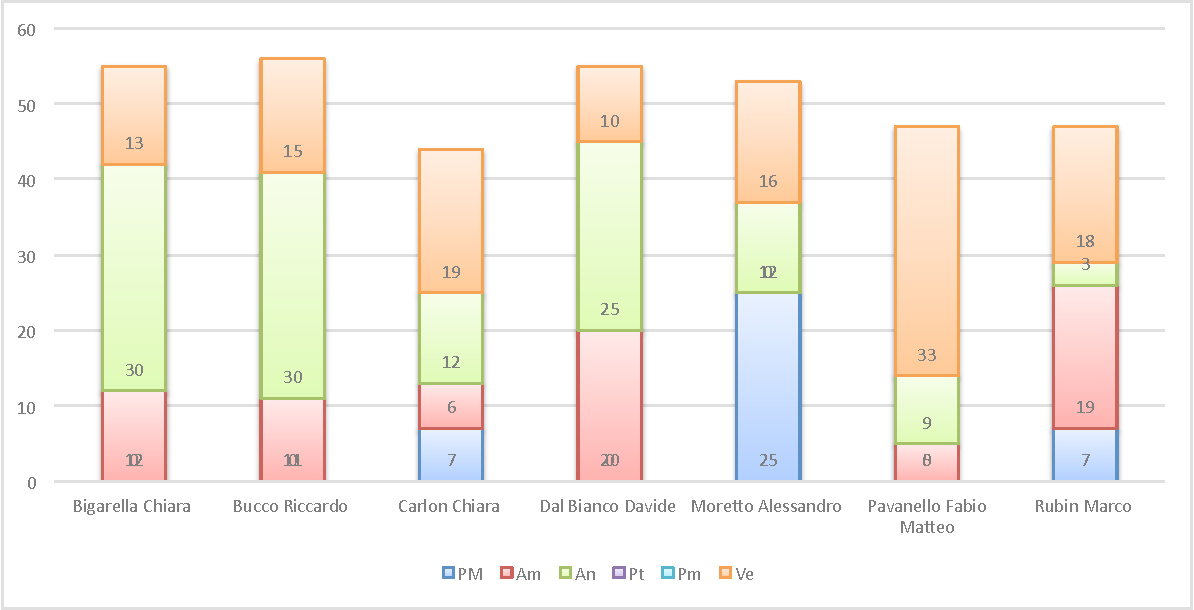
\includegraphics[width=\textwidth]{PianoDiProgetto/Pics/ChartOreInvest.png}
					\caption{Bar Chart ore totali di investimento}
				\end{figure}
			\paragraph{Prospetto economico}
				L'investimento per ogni ruolo è il seguente:
				\begin{table}
					\begin{center}
						\begin{tabular}{| l | c | c |}
							\hline
							Ruolo 				& Ore 		& Costi  \\ \hline
							
							Product Manager		& 39 		& \euro{} 1170 	\\
							Amministratore 		& 73 		& \euro{} 1460 	\\
							Analista	 		& 121 		& \euro{} 3025 	\\
							Progettista 		& - 		& \euro{} -  	\\
							Programmatore		& - 		& \euro{} - 	\\
							Verificatore		& 124 		& \euro{} 1860 	\\ \hline \hline
							
							Totale	 			& 357 		& \euro{} 7515 	\\ \hline
						\end{tabular}
					\end{center}
					\caption{Investimento per ruolo}
				\end{table}
				Riassumendo le ore di investimento per ruolo con un Cake Chart:
				\begin{figure}\centering
					%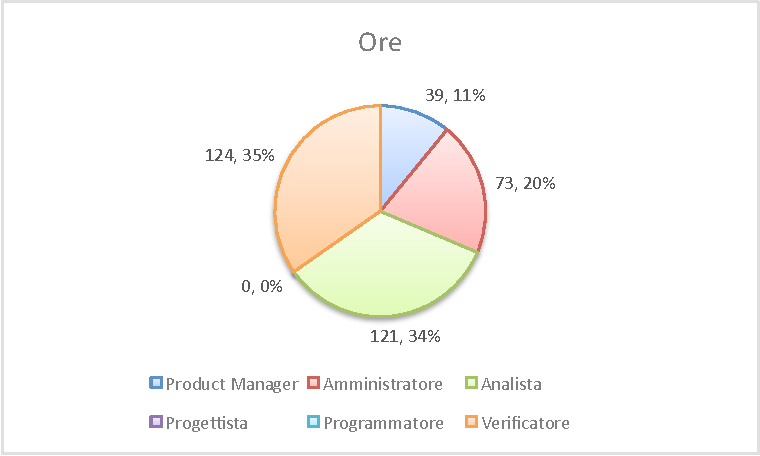
\includegraphics[width=\textwidth]{PianoDiProgetto/Pics/ChartTotOreInvest.png}
					\caption{Cake Chart ore di investimento}
				\end{figure}
				Riassumendo i costi per ruolo con un Cake Chart:
				\begin{figure}\centering
					%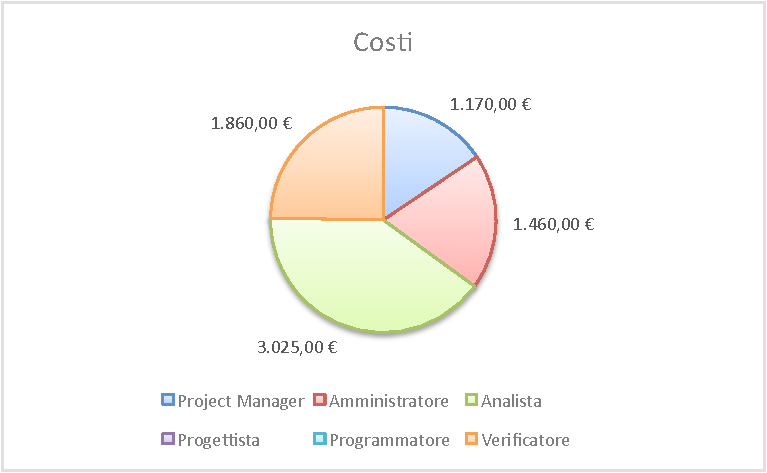
\includegraphics[width=\textwidth]{PianoDiProgetto/Pics/ChartTotCostiInvest.png}
					\caption{Cake Chart investimento per ruolo}
				\end{figure}
		\subsubsection{Ore rendicontate}
			Le ore rendicontate sono le ore svolte a carico del proponente.
			\paragraph{Suddivisione lavoro}
				La suddivisione delle ore rendicontate per ruolo di ogni componente del gruppo \groupname{} saranno le seguenti:
				\begin{table}
					\begin{center}
						\begin{tabular}{| l | c | c | c | c | c | c | c |}
							\hline
							Componente 					& PM		& Am 		& An 		& Pt 		& Pm 		& Ve 		& Ore Totali componente \\ \hline
							
							Bigarella Chiara 			& 10 		& - 		& 10 		& 32 		& 24 		& 29 		& 105 \\
							Bucco Riccardo 				& 15 		& - 		& - 		& 26 		& 26		& 38 		& 105 \\
							Carlon Chiara	 			& 10 		& 14 		& 25 		& 14 		& 15 		& 27 		& 105 \\
							Dal Bianco Davide 			& 17 		& - 		& - 		& 38 		& 23 		& 27 		& 105 \\
							Moretto Alessandro 			& - 		& 11 		& 23 		& 32 		& 20 		& 19 		& 105 \\
							Pavanello Fabio Matteo	 	& 13 		& - 		& 37 		& 9 		& 24 		& 22 		& 105 \\
							Rubin Marco					& 9 		& 7 		& 25 		& 23 		& 14 		& 27 		& 105 \\ \hline \hline
							
							Ore Totali Ruolo 			& 74 		& 32 		& 120 		& 174 		& 146 		& 189 		& 735\\ \hline
						\end{tabular}
					\end{center}
					\caption{Suddivisione ore totali rendicontate}
				\end{table}
				Riassumendo con un Bar Chart:
				\begin{figure}\centering
					%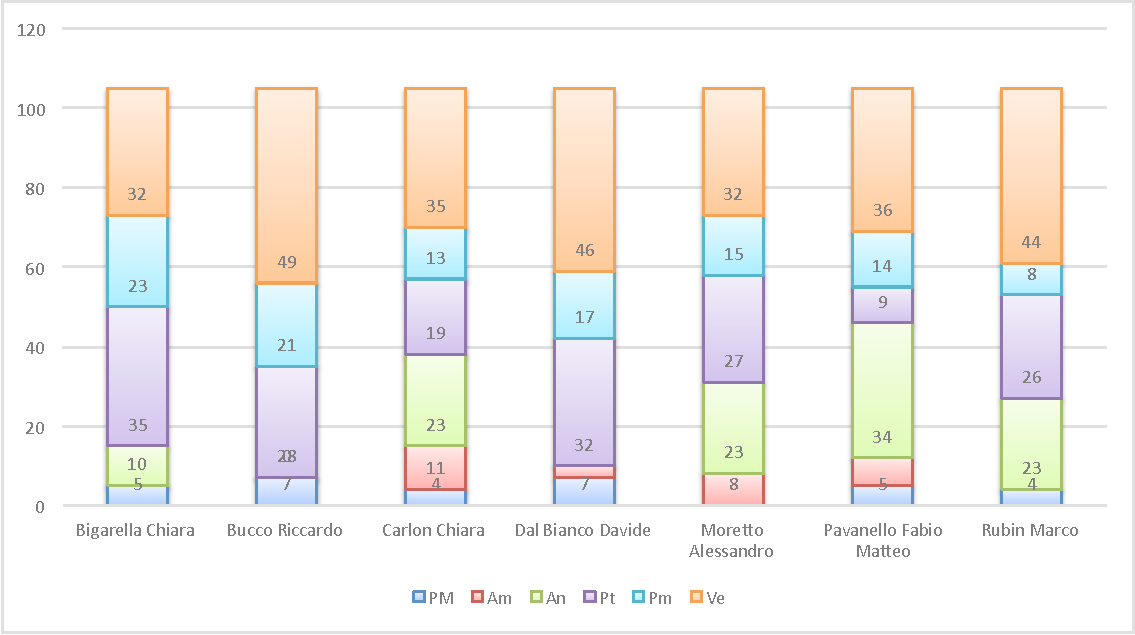
\includegraphics[width=\textwidth]{PianoDiProgetto/Pics/ChartOreRendic.png}
					\caption{Bar Chart ore totali rendicontate}
				\end{figure}
			\paragraph{Prospetto economico}
				Le ore rendicontate per ogni ruolo sono le seguenti:
				\begin{table}
					\begin{center}
						\begin{tabular}{| l | c | c |}
							\hline
							Ruolo 				& Ore 		& Costi  \\ \hline
							
							Product Manager		& 74 		& \euro{} 2220 	\\
							Amministratore 		& 32 		& \euro{} 640 	\\
							Analista	 		& 120 		& \euro{} 3000 	\\
							Progettista 		& 174 		& \euro{} 3828  	\\
							Programmatore		& 146 		& \euro{} 2190 	\\
							Verificatore		& 189 		& \euro{} 2835 	\\ \hline \hline
							
							Totale	 			& 735 		& \euro{} 14713 	\\ \hline
						\end{tabular}
					\end{center}
					\caption{Spese rendicontate per ruolo}
				\end{table}
				Riassumendo le ore rendicontate per ruolo con un Cake Chart:
				\begin{figure}\centering
					%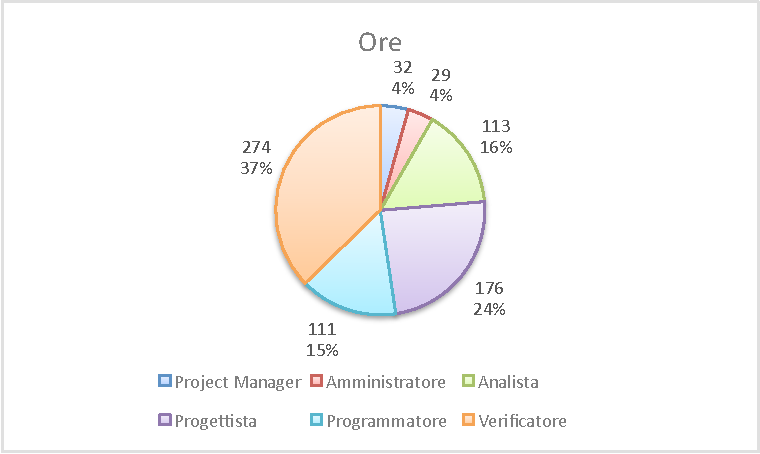
\includegraphics[width=\textwidth]{PianoDiProgetto/Pics/ChartTotOreRendic.png}
					\caption{Cake Chart ore rendicontate}
				\end{figure}
				Riassumendo i costi rendicontati per ruolo con un Cake Chart:
				\begin{figure}\centering
					%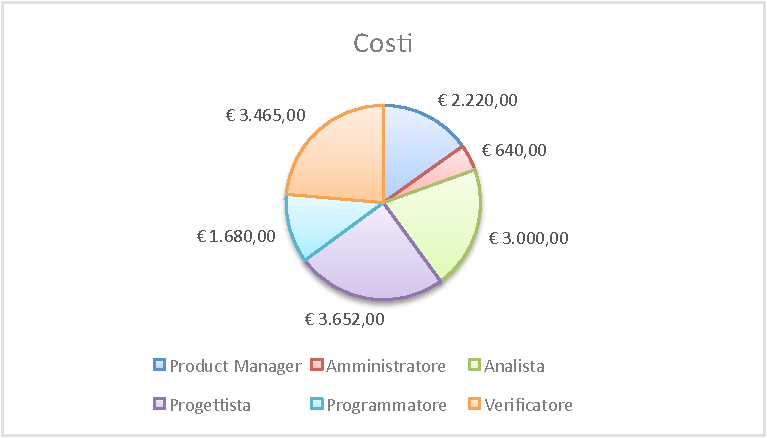
\includegraphics[width=\textwidth]{PianoDiProgetto/Pics/ChartTotCostiRendic.png}
					\caption{Cake Chart spese rendicontate per ruolo}
				\end{figure}
		\subsubsection{Conclusione}
			Il costo totale del progetto è di \euro{} 14713.
